\documentclass[a4paper, 11pt]{article}
\usepackage[utf8]{inputenc}
\usepackage[english]{babel}
\usepackage [autostyle, english = american]{csquotes}  % quote marks
\usepackage{mathpazo} % font families: charter, fourier, mathpazo, times
% \usepackage[UTF8]{ctex}

\usepackage[a4paper, centering]{geometry}
\geometry{left=2.5cm,right=2.5cm,top=2.5cm,bottom=2.5cm}   
% \geometry{a4paper, centering, scale = 0.85}

\usepackage{graphicx}
\graphicspath{ {images/} }

\usepackage{amsfonts}
%\usepackage{dsfonts}
\usepackage{amssymb}
\usepackage{amsmath}
\usepackage{verbatim}
\usepackage{amsthm}
\usepackage{mathrsfs}%花体字母

\usepackage{float}%used to place figure with specifier [H]
\usepackage{diagbox} % diagonal line in table
% \usepackage{bm} % bold symbol
\usepackage{tcolorbox}   % color box


%equation numbering associated with chapter/section
\numberwithin{equation}{section}

\usepackage{url}

% \usepackage[
% backend=biber,
% style=alphabetic,
% sorting=none
% ]{biblatex}
% \DeclareFieldFormat{eprint:arXiv}{%
%   arXiv: \href{https://arxiv.org/abs/#1}{#1}%
% }

% \addbibresource{ref.bib}
% % \bibliography{ref}   %  if backend = bibtex


% % if natbib is used
% %in the preamble
% %--------------------------------
\usepackage[square,numbers, compress]{natbib}
\bibliographystyle{apsrev4-1}   % unsrtnat, abbrvnat, plainnat
% \newcommand*{\doi}[1]{\href{http://dx.doi.org/#1}{doi: #1}}   % add hyperlink to doi
% \newcommand*{\eprint}[1]{\href{https://arxiv.org/abs/#1}{arXiv: #1}}   % add hyperlink to arXiv
% %--------------------------------
 
% %Where the bibliography will be printed
%   \bibliography{bibfile}


\usepackage{color}
\newcommand*{\red}{\textcolor{red}} %red text

\usepackage{hyperref}
\hypersetup{  colorlinks=true, linkcolor=blue, citecolor=red, urlcolor=blue  }

\usepackage{physics}
\usepackage{qcircuit}
\usepackage{subcaption} %for subfigure and subtable


\usepackage{amsthm}
\newtheorem{theorem}{Theorem}
\newtheorem{corollary}{Corollary}
\newtheorem{lemma}{Lemma}
\newtheorem*{remark}{Remark}
\newtheorem{conjecture}{Conjecture}
\newtheorem{proposition}{Proposition}

\theoremstyle{definition}
\newtheorem{definition}{Definition}


% \renewcommand{\bf}[1]{\mathbf{#1}}
% \renewcommand{\cal}[1]{\mathcal{#1}}
% \newcommand{\bb}[1]{\mathbb{#1}}
% \newcommand{\scr}[1]{\mathscr{#1}} %花体
% \renewcommand{\bold}[1]{\boldsymbol{#1}} % 数学符号和希腊字母的粗体
% \newcommand{\half}{\frac{1}{2}}
% \newcommand{\lbold}{\boldsymbol{\lambda}} % bold lambda
% \newcommand{\sign}{ {\rm sign} }
% \renewcommand{\bea}{\begin{align}}
% \renewcommand{\eea}{\end{align}}
% \newcommand{\ba}{\begin{eqnarray}}
% \newcommand{\ea}{\end{eqnarray}}
% \newcommand{\floor}[1]{\left\lfloor #1 \right\rfloor} % floor function
% \newcommand{\ceil}[1]{\left\lceil #1 \right\rceil} % ceiling function
% \renewcommand{\binom}[2]{%
% 	\left(%
% 	\substack{	#1 \\	#2}
% 	\right)%
% }   %   binomial coefficient
% \renewcommand{\P}{\mathcal{P}}
% \newcommand{\Q}{\mathcal{Q}}
% \newcommand{\R}{\mathcal{R}}
% \renewcommand{\S}{\mathscr{S}}
% \renewcommand{\a}{\vb{a}}
% \renewcommand{\b}{\vb{b}}
% \newcommand{\C}{\mathcal{C}}
% \newcommand{\U}{\mathcal{U}}
% \newcommand{\fracp}[2]{\left( \frac{#1}{#2} \right)} % fraction with parentheses
% \newcommand{\fracmp}[2]{\left( -\frac{#1}{#2} \right)} % fraction with parentheses and minus sign

% \def\s{\vb{s}}
% \def\promiseball{\textsc{PromiseBall}}
% \def\enc{\textsf{Enc}}
% \def\eval{\textsf{Eval}}
% \def\qball{\textsc{Qball}}


%\def\pgfsysdriver{pgfsys -dvipdfmx.def}
\usepackage{tikz}
\usetikzlibrary{positioning}
\usetikzlibrary{shapes.geometric}




\title{Code Documentation for HiQ Competition}
\author{Bin Cheng, Ximing Wang and Yuning Zhang}


\begin{document}
\maketitle

% \tableofcontents

\section{Problem 1}

The Hamiltonian is given by,
\begin{align}
H(s) = (1 - s)H_0 + s H_I \ ,
\end{align}
where 
\begin{align}
H_0 &= -B \sum_{k = 1}^N X_k \\
H_I &= -\alpha \sum_{k=1}^N X_k - \beta \sum_{k=1}^N Z_k - J \sum_{k = 1}^{N - 1} X_k X_{k + 1} - J \sum_{k = 1}^{N - 1} Z_k Z_{k + 1} \ ,
\end{align}
and $X_k$ and $Z_k$ are Pauli-$X$ and Pauli-$Z$ acting on the $k$-th qubit. Here, $N = 13$, $J = 2$, $\alpha = 0.5$, $\beta = 1.0$, $B = 0.5$ and $T = 3$. 

Let $s := t/T$ and $H(t) := (1 - t/T) H_0 + (t/T)H_1$. Then the evolution that we want to achieve is,
\begin{align}
\exp(-i \int_0^T H(t) \dd{t}) \ket{+}^{N} \ .
\end{align}
Such an evolution can be accomplished by Trotterization. First,
% \begin{align}
%     \int_0^T H(t) \dd{t} \approx \sum_{j = 0}^{M - 1} H(j \Delta t) \Delta t \ ,
% \end{align}
\begin{align}
    \int_0^T H(t) \dd{t} \approx \sum_{j = 0}^{M - 2} \frac{H(j \Delta t) + H( (j+1) \Delta t)}{2} \Delta t = \frac{H(0)}{2} \Delta t + \sum_{j = 1}^{M-2} H(j \Delta t) \Delta t + \frac{H(T)}{2} \Delta t \ ,
\end{align}
where $M = 21$ and $(M-1) \Delta t = T$, which implies $\Delta t = 3/20$. So we can implement the evolution operator by,
% \begin{align}
%     \exp(-i \sum_{j = 0}^M H(j \Delta t) \Delta t) &\approx \prod_{j = 0}^M e^{-i H(j \Delta t) \Delta t} \\
%     &\approx \prod_{j = 0}^M e^{-i (j \Delta t^2/T) H_I} e^{-i \Delta t (1 - j \Delta t /T) H_0} \ .
% \end{align}
\begin{align}
\exp(-i \int_0^T H(t) \dd{t}) &\approx e^{-i H(0) \Delta t /2} \prod_{j = 1}^{M-2} e^{-i H(j \Delta t) \Delta t} e^{-i H(T) \Delta t /2} \\
&\approx e^{-i H_0 \Delta t /2} \prod_{j = 1}^{M-2} e^{-i (j \Delta t^2/T) H_I} e^{-i \Delta t (1 - j \Delta t /T) H_0} e^{-i H_I \Delta t /2}
\end{align}

These operators can be decomposed into single- or two-qubit gates.
\begin{itemize}
    \item $j = 0$:
    \begin{align}
     e^{-i H_0 \Delta t /2} = \prod_{k = 1}^N e^{i B X_k \Delta t /2} 
     \end{align}
    
    \item $1 \leq j \leq M-2$: For the $H_0$ part, we have,
    \begin{align}
    e^{-i \Delta t (1 - j \Delta t /T) H_0} = \prod_{k = 1}^N e^{i B \Delta t (1 - j \Delta t /T) X_k} \ .
    \end{align}
    For the $H_I$ part, we have,
    \begin{align}
    e^{-i (j \Delta t^2/T) H_I} = & \prod_{k = 1}^N e^{i \beta (j \Delta t^2/T) Z_k} \prod_{k = 1}^{N-1} e^{i J (j \Delta t^2/T) Z_k Z_{k+1}} \\
    & \prod_{k = 1}^N e^{i \alpha (j \Delta t^2/T) X_k} \prod_{k = 1}^{N-1} e^{i J (j \Delta t^2/T) X_k X_{k+1}} \ .
    \end{align}
    Combining two parts, the evolution operator for the $j$-th time step is given by,
    \begin{align}
    & \prod_{k = 1}^N e^{i \beta (j \Delta t^2/T) Z_k} \prod_{k = 1}^{N-1} e^{i J (j \Delta t^2/T) Z_k Z_{k+1}} \\
    & \prod_{k = 1}^N e^{i \left( \alpha (j \Delta t^2/T) + B \Delta t (1 - j \Delta t /T) \right) X_k} \prod_{k = 1}^{N-1} e^{i J (j \Delta t^2/T) X_k X_{k+1}} \ .
    \end{align}

    \item $j = M-1$: 
    \begin{align}
    e^{-i (\Delta t /2) H_I} = & \prod_{k = 1}^N e^{i \beta (\Delta t /2) Z_k} \prod_{k = 1}^{N-1} e^{i J (\Delta t /2) Z_k Z_{k+1}} \\
    & \prod_{k = 1}^N e^{i \alpha (\Delta t /2) X_k} \prod_{k = 1}^{N-1} e^{i J (\Delta t /2) X_k X_{k+1}} \ .
    \end{align}
\end{itemize}



We apply these gates to the initial state $\ket{+}^N$ sequentially for $j = 0, 1, \cdots, 20$. Let the prepared state be $\ket{\psi}$. Then $E_D = \mel{\psi}{H_I}{\psi}$.

We implemented the circuit with ProjecQ engine and revoke the expectation measurement function in backend to get the corresponding energy after simulated annealing. 

The ideal ground state energy can be fairly approximated by setting the number of bins M in Trotterization to be sufficient large (100 as example).




\section{Problem 2}


The target of this task is to perform state preparation on restricted quantum
chips. Noting that the expressive power of a highly entangled parametrized
quantum circuit (PQC) is very strong. A sufficient number of ansatzs should
estimate any quantum states properly. To build up an highly entangled PQC, we
only need strong entangling gates between parameterized ansatzs.

In this case, the ansatz contains only single qubit quantum gates, which
doesn't depends on the connectivity of the quantum chips. Therefore, all we
need is to construct an entangling gate based on the topology of the chips.
For a fully connected quantum chip, a simplest idea is to connect each
neighboring qubits with a CNOT gate. But any Multilayer Parameterized Quantum
Circuits (MPQC) (see Fig.~\ref{fig:MPQC}) should work similarly. By the definition of MPQC, we need
$n-1$ CNOT gates that connects all qubits.


\begin{figure}[t]
    \centering
    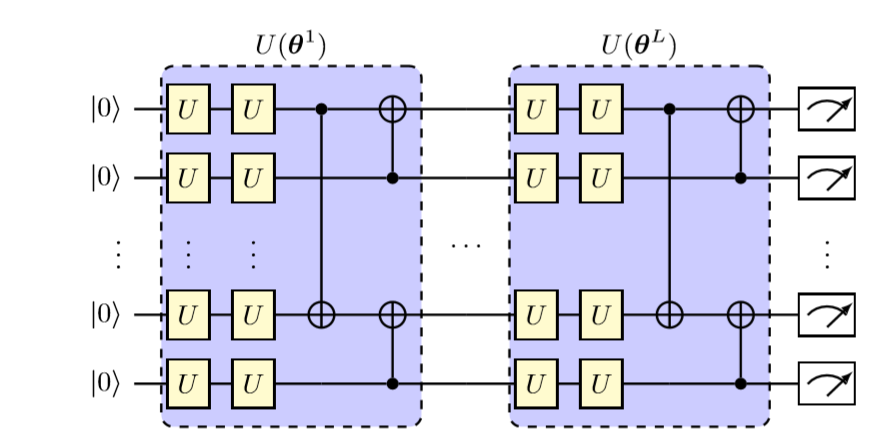
\includegraphics[width = 0.7\textwidth]{MPQC.png}
    \caption{MPQC. arXiv:1810.11922}
    \label{fig:MPQC}
\end{figure}



With restricted connectivity, a good idea is to centralize the CNOT gates on
qubits with high connectivity (so the entanglement spread fast). Therefore,
we can choose the qubit with highest connectivity as the control bit (root)
and performs CNOT with all its neighbors. Then we should choose the child
qubit connected to most untouched qubits and perform CNOT onto them.


\subsection{Cost function}

Suppose $\vb{a}$ is the target state vector. We separate its real and imaginary parts $\vb{a} = \vb{b} + i\vb{c}$, where $\vb{b}$ and $\vb{c}$ are real. Let $\vb{a}' = \vb{b}' + i\vb{c}'$ be our prepared state. Then we need to minimize $|\vb{b} - \vb{b}'|$ and $|\vb{c} - \vb{c}'|$. The distance $|\vb{b} - \vb{b}'|$ is defined as $\sqrt{\sum_i (b_i - b'_i)^2}$.




\section{Problem 3}

The basic idea of problem 3 is simple--with parameterized circuit, we can set a cost function to be the probability of given target state and tune the parameters to minimize the cost.

However, since the parameterized circuit, with 14 qubits width, contains more that 3000 quantum gates, the seems-easy problem can be actually hard to solve. Traditional optimization techniques based on cost and gradient evaluation require intensive computational resource and what's worse is these algorithms can't resist the attraction of local minimums. 
  

To handle this problem, we use a heuristic technique -- the Paricles Swarm Optimization (PSO) algorithm to avoid local minimum. This heuristic comes from an imitation of animal colony searching for food supply or water resources and is very strong against high-dimension complex problem.


In our instance, we initialized a PSO with 40 particles on given circuit to search for optimal parameters that maximize the target probability. 

The initial positions of particles are randomly set and generally with in 50 epoches we can achieve the required probability level. Typically this step will consume less than one hour since PSO is slow to converge.





% \printbibliography % if biblatex is used
% \bibliography{ref}

% \appendix

% \section{Appendix}



\end{document}
